
\begin{frame}{Shapley values}
    \begin{center}
    \begin{minipage}{0.4\textwidth}
    \begin{center}
 	   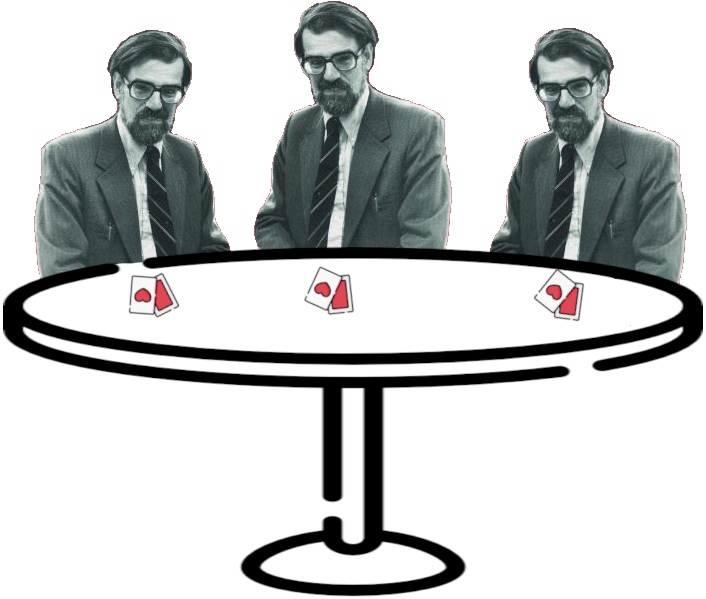
\includegraphics[width=0.9\linewidth]{fig/shapley-game.png}
    \end{center}
    \end{minipage}
    \begin{minipage}{0.55\textwidth}
    \begin{itemize}
        \item multi-player coalition game \gray{-- the players work together to gain the biggest reward they can}
        \item the reward is then divided between the players
    \end{itemize}
    \end{minipage}    
    \end{center}
    
    \textbf{Problem:} How to split the total payout (reward) between the players in \textbf{a fair way}, i.e. taking into consideration their contribution?

    \vspace{0.05in}  % THAT'S UGLY
    Shapley showed that there exists \textbf{a unique solution} to this problem.
    
    \note{
    \begin{itemize}
        \item oh, that's Shapley in the picture
        \item \textbf{multi-player coalition game} -- the players work together to gain the biggest reward possible
        \item the reward must be shared between the players -- so it's an additive feature attribution method (or additive player contribution distribution)
        \item how to do this in \textbf{a fair way}?
        \item Well, first we need to define mathematically, what does it mean 'a fair way'.
        \item And, BTW, Shapley has shown that there is \textbf{a unique way} of doing this, i.e. \textbf{a unique solution}
    \end{itemize}
    }
\end{frame}


\begin{frame}{The fairness properties}
    \begin{block}{\textbf{Efficiency}}
    The entire reward must be split.
     % The feature contributions must add up to the difference of the prediction for $x$ and the~\textbf<2>{average} prediction.
    
    % $\sum\nolimits_{j=1}^p\phi_j=\hat{f}(x)-E_X(\hat{f}(X))$
    \end{block}
    
    % \uncover<2->{
    \begin{block}{\textbf{Symmetry}}
    If two players contributed equally then their payout should be the same.
    
    % The contributions of two feature values $j$ and $k$ should be the same if they contribute equally to all possible coalitions.
    
    % If $val(S\cup\{x_j\})=val(S\cup\{x_k\})$
    % for all
    % $S\subseteq\{x_{1},\ldots,x_{p}\}\setminus\{x_j,x_k\}$
    % then
    % $\phi_j=\phi_{k}$
    \end{block}
    % }

    % \uncover<3->{
    \begin{block}{\textbf{Dummy}}
    A player who has no impact on the reward value gets no reward.
    
    % A feature $j$ that does not change the predicted value -- regardless of which coalition of feature values it is added to -- should have a Shapley value of $0$.    
    % If $val(S\cup\{x_j\})=val(S)$
    % for all
    % $S\subseteq\{x_{1},\ldots,x_{p}\}$
    % then
    % $\phi_j=0$
    \end{block}
    % }
    
    % \uncover<4->{
    \begin{block}{\textbf{Additivity}}
    If players play one game after another then calculating their rewards after each game should give the same result as calculating their total rewards once, after the last game.
    
    % For a game with combined payouts $val+val^+$ the respective Shapley values are as follows:
    % $\phi_j+\phi_j^{+}$
    \end{block}
    % }

    \note{
    \AW{I'm rewritting these properties to be less mathematical. We'll get lost in the details later. And this is when we'll deal with that and see how much simplification is allowed.}
    \AW{the cat working example already requires the notion of ALL coalitions}
    \begin{itemize}
        \item Once these properties are properly, mathematically defined, it turns out (i.e. Shapley has shown) that there is a unique solution.
        \item This means that splitting the reward with any other way than Shapley values breaks at least one of these properties, and thus, is unfair.
    \end{itemize}
    }
    
\end{frame}



\begin{frame}{The unique solution}
     \textbf{Definition:} The Shapley value is the average marginal contribution of a feature value across all possible coalitions.
    
    % The Shapley value of a feature value is its contribution to the payout, weighted and summed over all possible feature value combinations:
    
    % \begin{equation*}
    % \phi_j(val)=\sum_{\color<2->{cinnamon}{S\subseteq\{x_{1},\ldots,x_{p}\}\setminus\{x_j\}}} \frac{|S|!\left(p-|S|-1\right)!}{p!}\left(val\left(S\cup\{x_j\}\right)-val(S)\right)    
    % \end{equation*}

    
    % \begin{equation*}
    % \footnotesize
    % \phi_j(val)=
    % {\sum_{
    % \underbrace{S\subseteq\{x_{1},\ldots,x_{p}\}}_{\substack{\uparrow \\ \text{all possible coalitions} \\ \text{of $p$ players}}}
    % \underbrace{\setminus\{x_j\}}_{\substack{\uparrow \\ \text{without} \\ \text{player $j$}}}
    % }  % end \sum
    % }  % end \sum description 
    % \frac{
    % \overset{\substack{\text{no. of sequences}\\ \text{of players from $S$}\\\downarrow}}{|S|!}
    %  \overset{\substack{\text{no. of sequences of}\\ \text{the remaining players}\\\downarrow}}{\left(p-|S|-1\right)!}}
    % {\underset{\substack{\uparrow \\ \text{no. of sequences} \\ \text{of all players}}}{p!}}
    % \left(
    % \underbrace{val\left(S\cup\{j\}\right)}_{\substack{\uparrow \\ \text{reward with player $j$ present} \\ \text{player $j$}}}
    % -
    % \underbrace{val(S)}_{\substack{\uparrow \\ \text{ reward without} \\ \text{player $j$}}}\right)
    % \end{equation*}

    \begin{equation*}
    \phi_j(val)=
    {\sum_{
    \underbrace{S\subseteq\{x_{1},\ldots,x_{p}\}}_{\substack{\uparrow \\ \text{all possible coalitions} \\ \text{of at most $p$ players}}}
    \underbrace{\setminus\{x_j\}}_{\substack{\uparrow \\ \text{without} \\ \text{player $j$}}}
    }  % end \sum
    }  % end \sum description 
    \underbrace{\frac{|S|!(p-|S|-1)!}{p!}}_{\substack{\uparrow \\ \text{weighting factor}}}
    \underbrace{
    (
    \overbrace{val(S\cup\{j\})}^{\substack{\text{reward with} \\ \text{player $j$ present} \\ \downarrow }} 
    - \overbrace{val(S)}^{\substack{\text{reward without} \\ \text{player $j$} \\ \downarrow }} )
    }_{\substack{\uparrow \\ \text{$j$'s contribution for coalition $S$} }}
    \end{equation*}

    \note{
    \begin{itemize}
        \item read the definition
        \item \textbf{explain: marginal contribution} -- contribution of the player regardless of other players
        % (wiki) In probability theory and statistics, the marginal distribution of a subset of a collection of random variables is the probability distribution of the variables contained in the subset. It gives the probabilities of various values of the variables in the subset without reference to the values of the other variables.
        % so we want contribution of the player regardless of other players
        \item \textbf{explain: coalition} -- a subset of players
        % \item \textbf{note: across all possible coalitions} -- so over all sequences
        % \item note: average -- and we'll have to do some averaging
        \item warn that we will now express it mathematically
        \item go through the equation step by step
        \item \textbf{the contribution of player $j$} is the difference between the reward with him playing and the reward without him playing
        
        \item OK, on the following slides we'll discuss the weighting factor
    \end{itemize}
    }

\end{frame}

\begin{frame}{Order matters}
    \footnotesize
    Order matters when the function is nonlinear or the variables are not independent.

    \textbf{Nonlinearity:} let's go back to our AND example. A = 0, B = 1
    \begin{itemize}
        \item if we learn about A first, then it gets the entire contribution -- we already know what would be the answer -- and so B will get 0 contribution
        \item but if we learn first about B, then we still don't know what the answer would be -- thus A and B will get equal contribution
    \end{itemize}

    \textbf{Dependent variables:}
    \begin{itemize}
        \item we have four variables: A, B, C, D; B = C + D (so B and C, and B and D are dependent)
        \item we predict the sum of all the variables
        \item if we learn about the variables in order: A, B, C, D; then C and D have no contribution -- once we know A and B, we know that the sum is A + 2B
        \item if we learn about the variables in order: A, C, D, B, then C and D have nonzero contribution, but B has zero contribution -- once we learn about A, C, D, we know that the sum is A + 2 * (C + D)
    \end{itemize}

    When calculating Shapley values, all possible orderings are considered and an average contribution is calculated.

    \note{
    Which ordering to choose when calculating contribution? The answer is to consider all of them.
    }
\end{frame}

\begin{frame}{Weighting factor for a coalition of players}
    When calculating $j$'s contribution for some coalition $S$ we need to know how many sequences correspond to this situation:

    \begin{itemize}
        \item $|S|$ players can be ordered in $|S|!$ sequences
        \item the remaining players can be ordered in $(p - |S| - 1)!$ sequences
        \item coalition $S$ corresponds to $|S|!(p - |S| - 1)!$ sequences
    \end{itemize}

    There are $p!$ sequences of $p$ players, so each sequence has weight $\frac{1}{p!}$

    Therefore, the weight for $j$'s contribution to coalition $S$ is:
    $$\frac{|S|!(p - |S| - 1)!}{p!}$$

    % Molnar: Intuitive understanding of Shapley values
    % The feature values enter a room in random order. All feature values in the room participate in the game (= contribute to the prediction). The Shapley value of a feature value is the average change in the prediction that the coalition already in the room receives when the feature value joins them.

    \note{
    OK, so order matters. But we would like to use subsets not sequences but subsets are unordered. So... we need to employ some combinatorics!
    }
\end{frame}


